\documentclass[12pt]{article}
\usepackage[utf8]{inputenc}
\usepackage[brazilian]{babel}
\usepackage{hyperref}
\usepackage{lipsum}
\usepackage{geometry}
\usepackage[skip=5pt plus1pt, indent=20pt]{parskip}
\usepackage{indentfirst}
\usepackage{graphicx}
\usepackage[center]{caption}
\usepackage[font=small]{caption}
\usepackage{subcaption}
\usepackage{placeins}
\usepackage{setspace}
\usepackage{amsthm,amssymb,amsmath}
\usepackage{algorithm}
\usepackage{algpseudocode}

\renewcommand*\familydefault{\sfdefault} 

\graphicspath{{./midia/}}

\geometry{margin=2cm}

\title{\textbf{Trabalho Prático 2 - Desemprego}}
\author{\textbf{Lucas Almeida Santos de Souza - 2021092563\textsuperscript{1}}}
\date{\parbox{\linewidth}{\centering%
	\textsuperscript{1}Universidade Federal de Minas Gerais (UFMG)\endgraf
	Belo Horizonte - MG - Brasil\endgraf\bigskip
	\href{mailto:luscaxalmeidass@ufmg.br}{luscaxalmeidass@ufmg.br}}}

\begin{document}

\maketitle

%%%%%%%%%%%%%%%%%%%%%%%%%%%%%%%%%%%%%%%%%%%%%%%%%%%%%%%%%%%%%%%%%%%%%%%%%%%%%%

\section{Introdução}

	\par O trabalho consiste na resolução de um problema do tipo Casamento Estável, onde é preciso encontrar o melhor modo de combinar pessoas com as vagas das empresas onde elas se qualificam. Devem ser feitos dois algoritmos: um algoritmo guloso, onde a primeira solução encontrada será tomada, e não há arrependimentos; e um algoritmo ótimo, que encontre o máximo de pares pessoa-empresa possível dadas as qualificações.

	\par A entrada do programa desenvolvido consiste de um arquivo em que a primeira linha contém o número U de pessoas, o número J de empresas e o número E de qualificações pessoa-empresa, separados por espaço. As próximas E linhas do arquivo contém as qualificações, com o nome da pessoa e o nome da empresa separados por espaço. A saída do programa é apenas um número que indica o número máximo de pessoas que podem ser alocadas.

\section{Modelagem}

	\par Para facilitar a implementação dos algoritmos, logo na entrada os nomes das pessoas e empresas são convertidos para identificadores únicos, que são números inteiros. Esses identificadores são usados para indexar as estruturas de dados que representam o grafo. Isso é possível pois a solução do problema requer apenas o número de alocações realizadas, e não exige que sejam mostradas as alocações em si.

	\subsection{Algortimo Guloso}
		\par Para cada um dos algoritmos, foi pensada uma forma diferente de representar o grafo que modela o problema. Para o algoritmo guloso, foi utilizada uma matriz de adjacências, onde cada linha representa uma pessoa e cada coluna representa uma empresa. O valor da matriz na posição \texttt{(i, j)} é 1 se a pessoa \texttt{i} está qualificada para a empresa \texttt{j} e 0 caso contrário. Podemos ver um exemplo dessa representação abaixo:

		\begin{figure}[H]
			\centering
			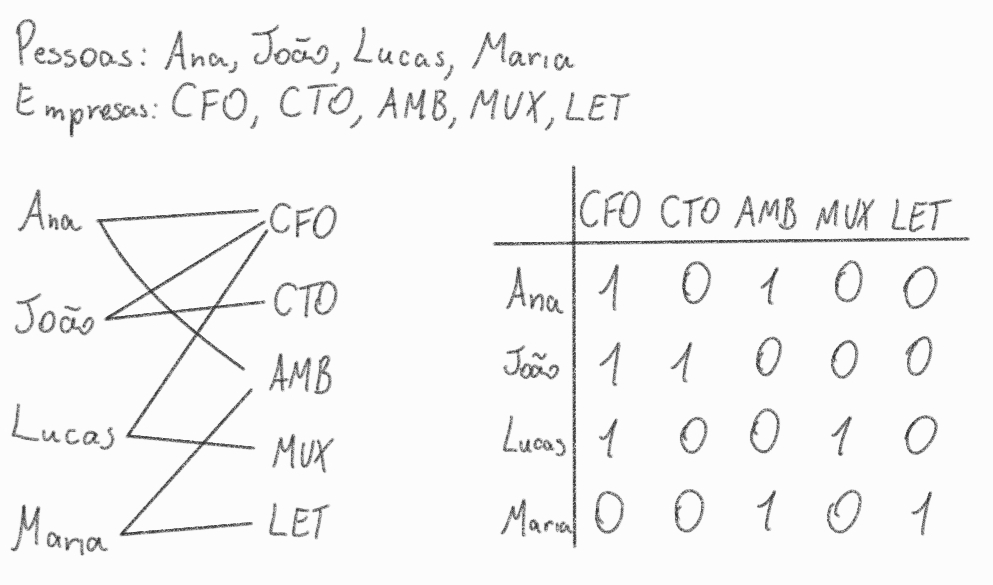
\includegraphics[width=0.8\textwidth]{exemplo_matriz.jpg}
			\caption{Representação da estrutura do grafo em matriz de adjacências}
			\label{exemplo_matriz}
		\end{figure}

		\par O algoritmo guloso é bem simples. Ele apenas percorre a matriz de adjacências, procurando a primeira vaga livre para cada usuário. Se ele encontra, a vaga é preenchida e temos mais uma alocação no contador. Dado $U$ como número de pessoas ou usuários e $J$ como número de vagas ou empresas, a complexidade desse algoritmo é $O(U \cdot J)$, pois ele percorre a matriz de adjacências uma vez para cada usuário e, no pior caso, percorrerá todas as vagas para cada usuário. Podemos ver o pseudocódigo abaixo:
		
		\vspace{12pt}
		\hrule
		\vspace{3pt}
		\hrule
		\noindent\textbf{resultadoGuloso( ):} \\
		\noindent\begin{tabular}{l}
			resultado := 0 \\
			vagas := [false] \footnotesize \textit{// Vetor de tamanho J inicializado com false, indica se uma vaga já foi preenchida} \\
			\textbf{para cada} usuário U \textbf{faça} \\
			\indent empresa := -1 \\
			\indent \textbf{para cada} empresa J \textbf{faça} \\
			\indent \indent \textbf{se} o usuário U está qualificado para a empresa J e ela não está ocupada \textbf{faça} \\
			\indent \indent \indent empresa := J \\
			\indent \indent \indent break \footnotesize \textit{// Encontrei a primeira empresa livre, não preciso mais procurar} \\
			\indent \indent \textbf{fim se} \\
			\indent \textbf{fim para cada} \\ \\
			\indent \textbf{se} empresa != -1 \textbf{faça} \footnotesize \textit{// o usuário foi aceito por alguma empresa} \\
			\indent \indent vagas[empresa] := true \footnotesize \textit{// a vaga foi preenchida} \\
			\indent \indent resultado++ \\
			\indent \textbf{fim se} \\
			\textbf{fim para cada} \\ \\
			\textbf{retorne} resultado
		\end{tabular}
		\hrule
		\vspace{3pt}
		\hrule
		\vspace{12pt}

		\par Esse algoritmo não é o algoritmo ótimo para o problema, pois ao escolher a primeira vaga disponível para algum usuário, ele não leva em consideração outros usuários que possam ter aquela vaga como única opção. Por exemplo, na entrada de teste abaixo, como o programa escolhe a primeira opção disponível, ele alocaria o Bruno na empresa RED, impedindo que Pedro pege essa vaga, que era a única qualificada para ele. Assim, o algoritmo guloso retornaria 4, enquanto o ótimo retornaria 5, pois alocaria o Bruno para a SWE, liberando a vaga da RED para o Pedro.

		\begin{figure}[H]
			\centering
			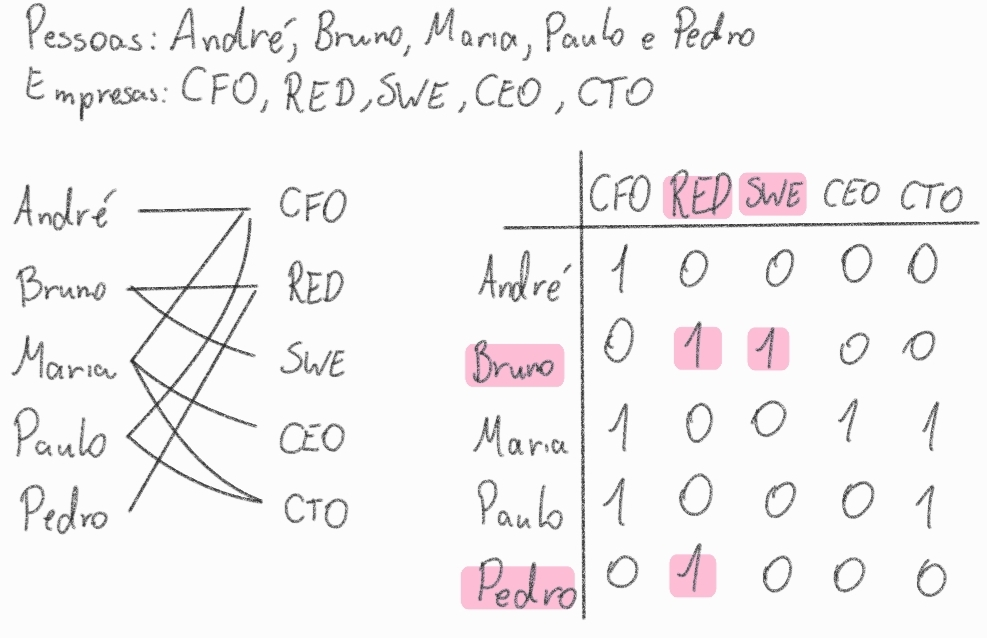
\includegraphics[width=0.8\textwidth]{exemplo_entrada.jpg}
			\caption{Exemplo de entrada que o algoritmo guloso não consegue resolver de maneira ótima}
			\label{exemplo_entrada}
		\end{figure}

	\subsection{Algoritmo Ótimo}

		\par Para o algoritmo ótimo, foi utilizado o conceito de fluxo máximo. Para encontrar o máximo de alocações possíveis, foi criado um grafo em forma de lista de adjacências, onde tanto as pessoas quanto as empresas são vértices, e a direção das arestas é sempre de pessoa para empresa. Além disso, foram adicionados dois novos vértices: a origem e o destino. A origem tem arestas para todas as pessoas e o destino recebe arestas de todas as empresas. As arestas não tem atributo de capacidade, pois todas as arestas têm capacidade 1, ou seja, durante a implementação do algoritmo de Ford Fulkerson, no grafo residual, uma aresta recém atravessada por um fluxo terá seu sentido invertido, em vez de simplesmente subtrair o fluxo passado. Podemos ver um exemplo dessa representação abaixo:

		\begin{figure}[H]
			\centering
			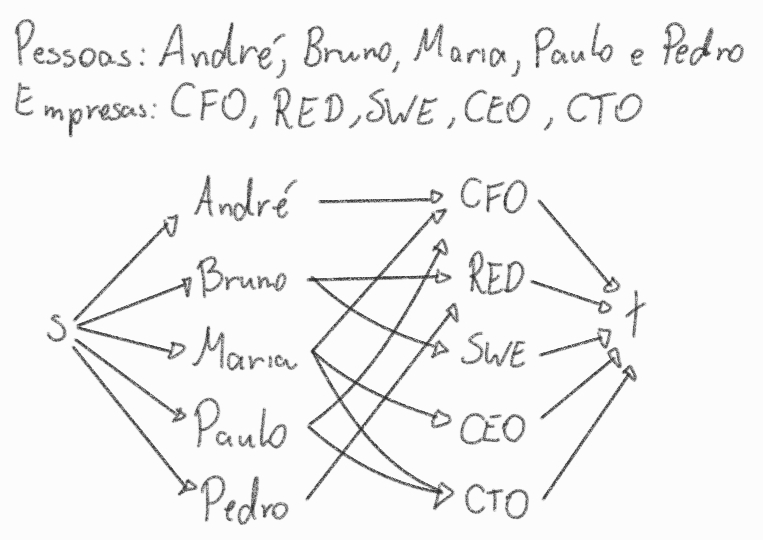
\includegraphics[width=0.6\textwidth]{exemplo_grafo.jpg}
			\caption{Representação da estrutura do grafo para algoritmo de fluxo}
			\label{exemplo_grafo}
		\end{figure}

		\par A função inicia criando o grafo para o algoritmo de Ford Fulkerson, adicionando as arestas direcionadas e os vértices origem e destino. Após isso, o algoritmo de Ford Fulkerson é chamado, retornando o fluxo máximo encontrado. Como o fluxo máximo é o número de alocações possíveis, esse valor é retornado como resultado. Esse algoritmo leva um tempo $O(U + J + U \cdot J)$ para preparar o grafo, e um tempo $O(E \cdot f)$ - onde $E$ é o número de relações de qualificação pessoa-empresa e $f$ é o fluxo máximo encontrado pelo algoritmo - para encontrar o fluxo máximo, resultando em uma complexidade total de $O(U \cdot J + E \cdot f)$. Contudo, o fluxo máximo que podemos atingir é $min(U, J)$, pois ao final do programa no melhor caso todas as pessoas ou empresas estarão alocadas. Além disso, o número de relações de qualificação pessoa-empresa é $U \cdot J$, pois, em um grafo bipartido completo, cada pessoa pode ser qualificada para todas as empresas, e cada empresa pode qualificar todas as pessoas. Assim, a complexidade final do algoritmo é $O(U \cdot J + U \cdot J \cdot min(U, J))$, que pode ser simplificada para $O(U \cdot J \cdot min(U, J))$, ou $O(U^2 \cdot J + U \cdot J^2)$.

		\par Como o algoritmo de Ford Fulkerson é bastante conhecido, o pseudocódigo abaixo mostra apenas a função que prepara o grafo para o algoritmo de fluxo:
		
		\vspace{12pt}
		\newpage
		\hrule
		\vspace{3pt}
		\hrule
		\noindent \textbf{resultadoOtimo( ):} \\
		\noindent\begin{tabular}{l}
			grafo := U + J + 2 \footnotesize \textit{// grafo de tamanho u+j+2, por causa de vértices fonte e sumidouro} \\ \\
			\textbf{para cada} usuário a \textbf{faça:} \\
			\indent grafo[0] $->$ grafo[a+1] \footnotesize \textit{// vértice fonte aponta para todos os usuários} \\
			\textbf{fim para cada} \\ \\
			\textbf{para cada} empresa b \textbf{faça:} \\
			\indent grafo[b+U+1] $->$ grafo[U+J+1] \footnotesize \textit{// todas as empresas apontam para o vértice sumidouro} \\
			\textbf{fim para cada} \\ \\
			\textbf{para cada} usuário a \textbf{faça:} \\
			\indent \textbf{para cada} empresa b \textbf{faça:} \\
			\indent \indent \textbf{se} usuárioQualificado(a, b) \textbf{então:} \\
			\indent \indent \indent \footnotesize \textit{// se o usuário a é qualificado para a vaga b, cria uma aresta de a para b} \\
			\indent \indent \indent grafo[a+1] $->$ grafo[b+U+1] \\
			\indent \indent \textbf{fim se} \\
			\indent \textbf{fim para cada} \\
			\textbf{fim para cada} \\ \\
			\textbf{retorne} fluxoMaximo(grafo, 0, U+J+1) \footnotesize \textit{// chama o algoritmo de Ford Fulkerson} \\
		\end{tabular}
		\hrule
		\vspace{3pt}
		\hrule

	\subsection{Conclusão}
		\par Podemos concluir que o algoritmo guloso é uma boa opção para uma primeira implementação, pois ele tem uma complexidade de ordem menor que o algoritmo ótimo, e, em muitos casos, ele consegue encontrar a solução ótima, tendo alcançado uma precisão de 94\% nos 13 testes de caso entregues. Contudo, o algoritmo guloso não é capaz de encontrar a solução ótima para todos os casos, como podemos ver no exemplo da figura \ref{exemplo_entrada}. Assim, o algoritmo ótimo é necessário para encontrar a solução ótima para todos os casos, e, apesar de ter uma complexidade maior, ele passou por todos os testes de caso em um tempo razoável.
\end{document}